\documentclass{report}
\usepackage{graphicx}

\begin{document}

\title{Thesis Proposal}
\author{Adam Yedidia}

\maketitle

\begin{abstract}
For my thesis, I propose to write a general-purpose compiler from a programming language of my design to a single-tape, two-symbol Turing machine with as few states as possible. Once this is complete, I propose to write a program in my language that will verify the consistency of Zermelo-Fraenkel set theory (or ZFC), and compile that program down into a Turing machine description. In so doing, I will have created a description for a Turing machine whose behavior cannot be predicted by ZFC. This is true by inspection, because since a logic system cannot prove its own consistency, a logic system cannot prove whether or not a Turing machine that verifies its consistency accepts or rejects.
\end{abstract}

\section{Introduction}
The work of my thesis would not have been possible without first splitting it into two parts: the construction of the compiler, and the 

\chapter{The Compiler}

The compiler used and referenced in this paper has as its goal to convert a program written in TMD into a description of Turing machine running on a single tape and using a 2-symbol alphabet. In between, the code is passed through two intermediate stages: a description of a Turing machine running on multiple tapes using a 3-symbol alphabet, and a description of a Turing machine running on a single tape using a 4-symbol alphabet. A detailed diagram illustrating this process is visible in Figure~\ref{fig:process}. \\

In this chapter, each of the four representations will be described in turn, from highest- to lowest-level. Additionally, detailed explanations will be given for how the conversion of one representation to the one immediately below it is done.

\section{TURD} 

\begin{figure} 
\begin{center} 
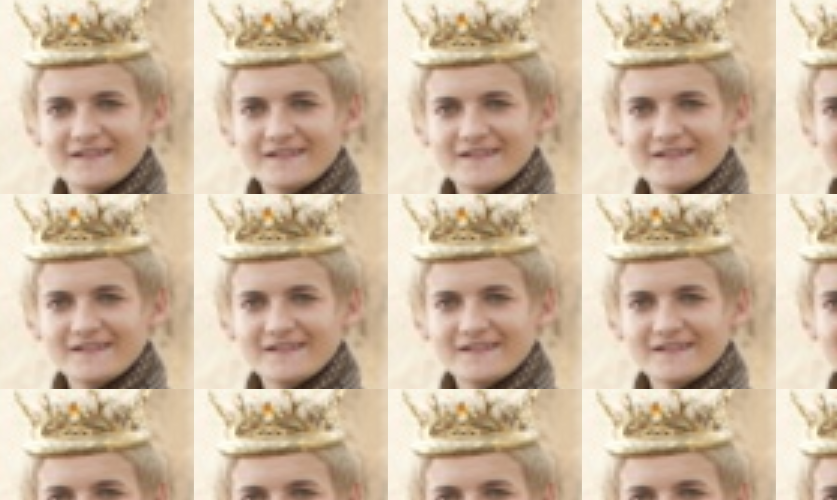
\includegraphics[height=2.5in,width=5in,angle=0]{many_joffrey_heads.png} 
\caption{This diagram illustrates each of the steps in the conversion between a program written in TMD and a description of a single-tape Turing machine with a binary tape alphabet.\label{fig:process}} 
\end{center} 
\end{figure}  


\end{document}

